% Kapanış sentezi: ölçtüğümüz her kaldıraç b = beta - 1 üzerinde, tek
% ölçekte, gözlemin kendi belirsizliğine karşı.
% `docs/rapor2204` içinden derle:  lualatex sekil/duyarlilik.tex
\documentclass[border=3pt,tikz]{standalone}
\usepackage{pgfplots}
\usepackage{pgfplotstable}
\usepackage{amsmath}
\usepackage[outline]{contour}
\usetikzlibrary{calc}
\pgfplotsset{compat=1.18}
\contourlength{1.0pt}
\tikzset{>=latex}

\makeatletter\newcommand{\pgfplotsdrawaxis}{\pgfplots@draw@axis}\makeatother
\pgfplotsset{axis line on top/.style={
  after end axis/.append code={\pgfplotsdrawaxis}}}

\colorlet{ink}{black!82}
\colorlet{infercol}{blue!55!cyan!75!black}  % öğrenmek istediğimiz
\colorlet{fixcol}{red!70!black}             % kararla sabitlediğimiz
\colorlet{obscol}{green!42!black}

% İçinde matematik taşıyan bir liste makroyla açıldığında girdi yığınını
% patlatıyor; liste doğrudan yazıldı.

\begin{document}
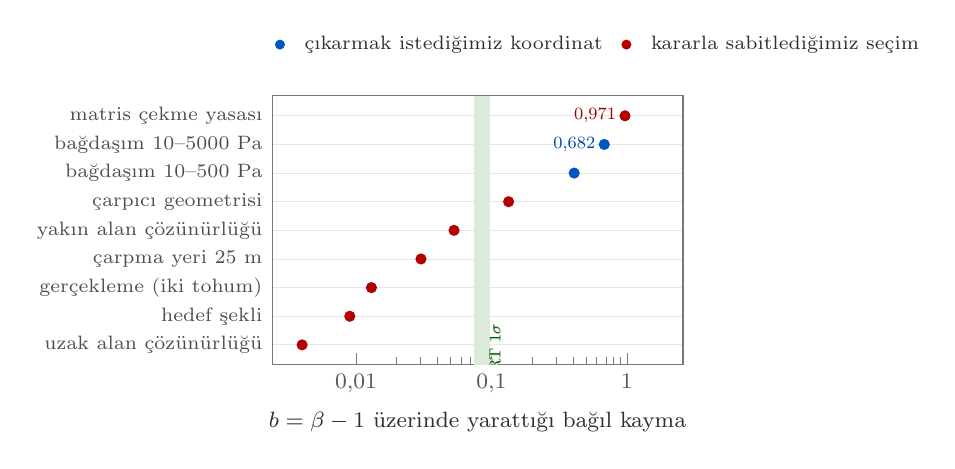
\begin{tikzpicture}[font=\footnotesize]
\begin{axis}[
  width=68mm, height=50mm,
  xmode=log, xmin=0.0024, xmax=2.6,
  ymin=-0.7, ymax=8.7,
  ytick={0,1,...,8},
  yticklabels={matris çekme yasası,bağdaşım $10$--$5000$ Pa,bağdaşım $10$--$500$ Pa,çarpıcı geometrisi,yakın alan çözünürlüğü,çarpma yeri $25$ m,gerçekleme (iki tohum),hedef şekli,uzak alan çözünürlüğü},
  y dir=reverse,
  yticklabel style={font=\scriptsize, text=ink!85},
  xlabel={$b=\beta-1$ üzerinde yarattığı bağıl kayma},
  xtick={0.01,0.1,1}, xticklabels={$0{,}01$,$0{,}1$,$1$},
  xtick pos=bottom, ytick pos=left,
  y axis line style={draw=none}, ytick style={draw=none},
  axis line style={draw=ink!65}, tick style={draw=ink!65},
  ticklabel style={text=ink!80},
  label style={text=ink},
  enlarge y limits=false,
  ymajorgrids, grid style={draw=ink!12, line width=0.3pt},
  % `axis line on top` eksenin tamamını -- ızgara dahil -- çizimlerden
  % SONRA yeniden çiziyor, bu da kılavuz çizgilerinin imleçleri kesmesine
  % yol açıyordu. Çerçeve buna değmez; eksen altta kalır.
  axis on top=false,
]

  % --- gözlemin kendi 1-sigma'sı, taban olarak -------------------------
  \fill[obscol!14] (axis cs:0.0740,-0.7) rectangle (axis cs:0.0972,8.7);
  % Etiket kısa: "b üzerinde DART 1-sigma" şeridin yüksekliğine sığmayıp
  % eksen tarafından kesiliyordu. Neyin üzerinde olduğu altyazıda yazılı.
  \node[scale=0.72, text=obscol!85!black, rotate=90, anchor=north]
       at (axis cs:0.086,8.55)
       {\contour{obscol!14}{DART $1\sigma$}};

  % --- kararla sabitlediklerimiz ---------------------------------------
  \addplot[only marks, mark=*, mark size=1.8pt, draw=fixcol, fill=fixcol]
    coordinates {(0.0040,8) (0.0090,7) (0.0130,6) (0.0302,5)
                 (0.0530,4) (0.1340,3) (0.9706,0)};

  % --- çıkarmaya çalıştığımız koordinat --------------------------------
  \addplot[only marks, mark=*, mark size=1.8pt,
           draw=infercol, fill=infercol]
    coordinates {(0.4088,2) (0.6820,1)};

  \node[scale=0.78, text=fixcol!85!black, anchor=east, inner sep=4pt]
       at (axis cs:0.9706,0) {\contour{white}{$0{,}971$}};
  \node[scale=0.78, text=infercol!85!black, anchor=east, inner sep=4pt]
       at (axis cs:0.6820,1) {\contour{white}{$0{,}682$}};

\end{axis}

\begin{scope}[shift={($(current axis.north west)+(1mm,6.5mm)$)}]
  \fill[infercol] (0,0) circle (1.8pt);
  \node[anchor=west, text=ink, font=\scriptsize, inner sep=3pt] at (2mm,0)
       {çıkarmak istediğimiz koordinat};
  \fill[fixcol] (44mm,0) circle (1.8pt);
  \node[anchor=west, text=ink, font=\scriptsize, inner sep=3pt] at (46mm,0)
       {kararla sabitlediğimiz seçim};
\end{scope}

\end{tikzpicture}
\end{document}
